\documentclass[letter,12pt]{article}
\usepackage[letterpaper,right=1in,left=1in,top=1in,bottom=1in]{geometry}
\usepackage{setspace}
\onehalfspacing

\usepackage[utf8]{inputenc}   % allows input of special characters from keyboard (input encoding)
\usepackage[T1]{fontenc}      % what fonts to use when printing characters       (output encoding)
\usepackage{amsmath}          % facilitates writing math formulas and improves the typographical quality of their output
\usepackage[hyphens]{url}     % adds line breaks to long urls
\urlstyle{tt}                 % how urls appear, options tt rm sf and same, see https://mirrors.mit.edu/CTAN/macros/latex/contrib/url/url.pdf
\usepackage[pdftex]{graphicx} % enhanced support for graphics
\usepackage{tikz}             % Easier syntax to draw pgf files (invokes pgf automatically)
\usetikzlibrary{arrows}

\usepackage{mathptmx}           % set font type to Times
\usepackage[scaled=.90]{helvet} % set font type to Times (Helvetica for some special characters)
\usepackage{courier}            % set font type to Times (Courier for other special characters)

% \usepackage[longnamesfirst, sort]{natbib}\bibpunct[]{(}{)}{,}{a}{}{;} % handles biblio and references 
\usepackage[sort]{natbib}\bibpunct[]{(}{)}{,}{a}{}{;} % handles biblio and references 

\usepackage{rotating}         % sideway tables and figures that take a full page
\usepackage{caption}          % allows multipage figures and tables with same caption (\ContinuedFloat)

\usepackage{dcolumn}          % needed for apsrtable and stargazer tables from R to compile
\usepackage{arydshln}         % dashed lines in tables (hdashline, cdashline{3-4}, 
                              %see http://tex.stackexchange.com/questions/20140/can-a-table-include-a-horizontal-dashed-line)
                              % must be loaded AFTER dcolumn, 
                              %see http://tex.stackexchange.com/questions/12672/which-tabular-packages-do-which-tasks-and-which-packages-conflict


\newcommand{\mc}{\multicolumn}

%% TO ADD NOTES IN TEXT, PUT % BEFORE THE ONE YOU WANT DISABLED
%\usepackage[disable]{todonotes}                            % no show
\usepackage[colorinlistoftodos, textsize=small]{todonotes} % show notes
\newcommand{\emm}[1]{\todo[color=red!15, inline]{\textbf{Eric:} #1}}

%% \usepackage{xr} % allows cross-ref to other file
%% \externaldocument{urge15appendix}

%% %for submission: sends figs, tables, and footnotes to last pages
%% \RequirePackage[nomarkers,nolists]{endfloat}     % sends tables and figures to the end
%% \RequirePackage{endnotes}                        % turns fn into endnotes; place \listofendnotes where you want 
%%                                                  %the endnotes to appear (it must be after the last endnote).
%% \let\footnote=\endnote
%% \newcommand{\listofendnotes}{
%%    \begingroup
%%    \parindent 0pt
%%    \parskip 2ex
%%    \def\enotesize{\normalsize}
%%    \theendnotes
%%    \endgroup
%% }

%% % for submission: drop page numbers when producing title page
%% \pagenumbering{gobble} % Remove page numbers (and reset to 1)
%% \pagenumbering{arabic}% Arabic page numbers (and reset to 1)

\setcitestyle{citesep={;}}

\usepackage{hyperref}

\usepackage{bigfoot}  %% allows the use of \verb command within footnotes

\begin{document}

\title{Local Competition in Mexican Politics: \\ A Comprehensive Dataset of Municipal Elections}
\author{Eric Magar \\ ITAM}
\date{\today}
\maketitle

\begin{abstract}
\noindent This note introduces a publicly-available dataset of municipal-level vote returns for Mexican municipal government elections between 1979 and 2025. It covers nearly 37,000 races and distributes municipal aggregates of the votes each party or coalition won, of void ballots, and of total votes cast; the number of eligible voters registered; the number of candidates competing and the winner's name; the election's date; and ancillary census bureau and election board municipality id codes for merging socio-demographic data and vote returns of other elections. The note presents sources, elaborates standardization of the time-series cross-section, and performs descriptive analysis showing both conformity of patterns in the data to received wisdom on Mexican elections. Descriptions demostrate several interesting uses of the data.
\end{abstract}

\noindent The advent of competition in Mexican politics produced a wealth of public data in most areas of government. A parallel boom occured naturally in the study of politics, policy, and process, in areas as diverse as the distributed data: poverty relief, decentralized spending, public health, education, infrastruture, special interest groups, organized crime, and much more.\footnote{See \citet{diaz-estevez-magaloni-Poverty-book.2016, delao.cctransfers.2013, cantuGroceries2019, hernandez.jaramillo.FiscalDescentralMx2008wd, king.etal.segPop.2007, frenk.2006, behrman.etal.Prospera2025qe, avitabile.dehoyos.2018, garfias.etal.Infrastructure2021, palmer.rubin.Patronage2019cps, dube.garcia.ponce-MaizeDrugs2016jeea, dell.DrugWar.2015aer}.}  While much of this analysis is at small units, such as firms, schools, census tracts, or even individuals, processes invariably intersect with municipal governments, and multivariate models typically include controls at this level. Municipal-level vote returns are therefore one key input for analysis. 

% \noindent The advent of competition in Mexican politics produced a wealth of public data in all areas of government. A parallel boom occured naturally in the study of politics, policy, and process, in areas as diverse as the data: poverty relief \citep{diaz-estevez-magaloni-Poverty-book.2016, delao.cctransfers.2013, cantuGroceries2019}, decentralized spending \citep{hernandez.jaramillo.FiscalDescentralMx2008wd}, public health \citep{king.etal.segPop.2007, frenk.2006}, education \citep{behrman.etal.Prospera2025qe, avitabile.dehoyos.2018}, infrastruture \citep{garfias.etal.Infrastructure2021}, interest groups \citep{palmer.rubin.Patronage2019cps}, organized crime \citep{dube.garcia.ponce-MaizeDrugs2016jeea, dell.DrugWar.2015aer}, and much more. While much of this analysis is at small units, such as firms, schools, census tracts, or individuals, processes invariably intersect with municipal government and politics, and multivariate models typically include controls at this level. Municipal-level vote returns are therefore one key input for analysis. 

This research note introduces a dataset of Mexican municipal election vote returns in recent decades. The dataset is distributed in a repository, publicly available at \url{https://github.com/emagar/elecRetrns}. Vote returns are information in the public domain that can be found in the web with relative ease. But primary sources are spread across state-by-state web sites, lack standardized reports, have many missing or incomplete years, and many are on the brink of being scrapped due to insufficient funding. The repository consolidates all this in a single source. 

The research note proceeds thus. Section 1 describes municipal government institutions. Section 2 briefly presents the main contenders in municipal party systems. Section 3 elaborates data coverage and its organization in the distributed files. Section 4 discusses the rising frequency of pre-lection coalitions in the units of observation. Section 5 performs descriptive analysis of key variables in the data, contrasting patterns to previous scholarship. Section 6 concludes.

\section{Municipal governments}
As of May 2025, Mexico's thirty-one states were subdivided into 2,460 municipalities, plus 17 municipality-equivalents in Mexico City, the nation's capital. \emph{Municipios} elect the bottom tier of governments in the federal system.
\subsection{Policy making and fiscal authority}
Municipal governments have constitutional authority over community police, zoning and construction permits, drinking water supply, sewerage and waste disposal, street lighting, pavement, and park management, and regulate public markets, slaughterhouses, and cemeteries. Elected municipal officers appoint municipal staff and subcontract services and personnel in order to undertake these responsibilities, and these are key sources of patronage in a spoils system. Local political organizations, and the resources they mobilize in pursuit of municipal office, are key to the maintenance of state and national parties \citep{coppedge.MxVen.1993, key.1964, rosas.lucardi.Brokers.2019}. 

 

Municipal governments raise property taxes only and collect fees for public services. Adding insult to the injury of a meager constitutional fiscal endowment, few municipalities in the past invested in the administrative structure for revenue collection \citep{garfias.state.cap.2018}. Most, especially in rural Mexico, obtain the lion's share of their financial resources from federal revenue sharing and earmarked federal investments \citep{diaz.cayeros.2006, figueroa-mansur-itam.2024}. Bureaucratic capacity varies widely. The median municipal government employed or hired 13 bureaucrats per 1,000 registered voters in 2023, just shy above the lower quartile's 9 or fewer. The top decile, with 32 or more bureaucrats per 1,000, was two and a half times above the median.\footnote{Descriptive statistics computed with data from the 2023 Municipal Government Census \citep{inegi.CensoGobMun2023}, excluding Mexico City and uneleted municipalities.}

\subsection{Government structure}\label{S:structure}
Municipal power is vested to a popularly-elected body, the \emph{Ayuntamiento} (literally `yoked together'). The council or \emph{cabildo} and a mayor (called \emph{presidente} in some states, \emph{primer regidor} in others) make up the Ayuntamiento, deciding by majority rule. The mayor is executive officer, presides municipal council sessions with voice and the tie-breaking vote, and holds variable municipal appointment powers \citep{robles-mtz.Municipio.2009, rmz-millan.2000}. Cabildo size is proportional to population. Precedence-ordered councilors (called \emph{regidores} or \emph{concejales}) propose and vote municipal policy through ordinances and rules. One or more \emph{síndicos}, officers in charge of the treasury and the municipio's legal representation, complete the council in some states. Síndicos may be elected or appointed. Appointed síndicos have voice but no vote in the council. Municipalities have no judicial power. States do.

I drop Mexico City from the descriptions below due to its special status (but it is included in the data). Before 1997, the mayor of the Federal District was a presidential appointee, who would in turn appoint delegates for the city's 16 administrative jurisdictions (called \emph{delegaciones}). Reformers made all these elected offices in 1997. The Federal District did not, however, gain status as a state, nor did delegación executives gain fiscal powers---taxation remains in the hands of the city executive. The city further reformed in 2018, adding councils to its quasi-municipalities (now called \emph{alcaldías}) and renaming the Federal District as Mexico City \citep{rabell.2017}. 

\subsection{Electoral institutions}
Presidents are elected by plurality. Regidores are elected in two groups: one group by plurality, the other by proportional representation (PR). The plurality-to-PR regidores ratio shifts considerably across states. As of 2010, the ratio in the mean Ayuntamiento was $2:1$. The state of Guanajuato's, with the lowest plurality share in the mix, had a $1:4$ ratio, while Tabasco's, with the highest, had a $4:1$ ratio \citep[][:14]{gil.2010}. With parity, the president controls the council majority.

This is always so because municipal officers are elected in fused tickets. Voters have a single vote, which they cast for a list of candidates including a municipal president at the top of the ticket, ranked regidores, and síndicos where applicable. The vote is fused \citep[see ][:42]{cox.1997} as it simultaneously affects the vote totals of candidates running for different offices: the presidency, all plurality regidores, and síndicos, where elected, are allocated to the most-voted list. Remaining regidores are distributed proportionally to the closed lists. Split ticket voting is therefore not technically possible.

\subsection{Exceptional electoral institutions}
Two notable exceptions are the states of Chihuahua since 1998 and Nayarit since 2008. Voters there have two votes, therefore opening up the possibility of split ticket voting. In Chihuahua, one vote elects the síndico by plurality, another elects the remaining municipal officers as described above (ratio $8:5$).

In Nayarit, one vote elects a president--síndicos fused ticket by plurality in municipio-wide elections. The second vote elects plurality regidores in single-member districts called \emph{demarcaciones}, into which municipios are subdivided for the purpose. Second votes are then pooled in a secondary district (the municipio as a whole) to distribute PR regidores to the closed lists. While the ratio in Nayarit is $7:3$, winning presidents could end up in the council minority unless their party secures enough district victories.

\subsection{Term limits}
Elected municipal officers have three-year terms.\footnote{Coahuila's Ayuntamientos elected between 2005 and 2013 (inclusive), Hidalgo's since 2016, and Veracruz's between 2013 and 2021 enjoyed four-year terms. Exceptional distortions to three-year terms also occurred whenever state electoral calendars changed, something quite common in the period. See \citet{magarInstReel.2017} and \url{https://github.com/emagar/calendarioReeleccion}.} Up to those with terms ending in 2017, all were single-term limited. To everyone's surprise, reformers removed Mexico's eighty-year old constitutional ban on consecutive reelection midway in the last decade. Counter-reformers restated the ban a decade later---so everyone elected in 2030 and after will, again, be single-term limited. In the interim, states could opt for two-term limits for municipal governments. All states except Hidalgo and Veracruz did so, the reform kicking off in the 2018 elections in twenty-three states. Incumbents in the other seven reforming states were gradually able to run again for office since.

%Up to those elected in 2017, all were single-term limited. And everyone elected in 2030 will again be single-term limited. To everyone's surprise, reformers removed Mexico's eighty-year old constitutional ban on consecutive reelection midway in the last decade. Counter-reformers restated the ban ten years later. In the interim, states could opt for two-term limits for municipal governments. All states except Hidalgo did so, the reform kicking off in the 2018 elections in twenty-three states. Incumbents in the other eight reforming states have been able to run again for office gradually since (the last will be Veracruz's in 2028). 


With a frankly conservative scope and very much illustrative of the notion of state irresoluteness \citep{cox.mccubbins.2001}, ephemeral reelection should nonetheless leave a systematic mark in municipal politics. Six consecutive years in office falls short of qualifying as the long haul, but doubling up Ayuntamientos' time horizons ought to encourage more enterprising policy. Much more fundamentally, the perspective of reelecting for another term should strongly incentivize ambitious mayors and regidores in the period to invest substantially in maintaining their electoral alliances alive and mobilized \citep{cain.etal.1987, motolinia-reel-pork2021}. Which, in turn, should systematically nurture a degree of responsiveness in municipal distributive politics \citep{cox.mccubbins.1986, jacobson.kernell.1983}. The reform, and its dismissal too, therefore offer a unique laboratory to study institutional change at the core of much political theory since \emph{The Federalist Papers} \citep{madison.etal.1788, mayhew.1974, schlesinger.1966, miller.hammond.1989}.

\subsection{Usos y costumbres}\label{S:uyc}

A final elaboration before moving on involves other observations dropped from the data. Of 570 municipalities in the state of Oaxaca, only 152 elect Ayuntamientos by popular vote. The rest, with predominantly indigenous populations, opted out of the electoral process since 1995, appointing authorities through tribal councils instead \citep[known as \emph{usos y costumbres} institutions, see][]{elizarraras.2002, eisenstadt.rios.uyc.2014}. Seven municipalities in three other states achieved the same status in the past decade. These 425 municipalities are removed from the dataset.\footnote{A note `To uyc in \emph{year}' indicates the period immediately before a municipality exits the electoral process and the time series in the dataset following this route.}

\section{The parties}

This section briefly describes the main parties in the period. All are national organizations that have have competed systematically in a fair number of municipal races throughout the period. BORROW THIS FROM CORNELIUS AND WELDON.

\subsection{Major parties}

\begin{description}
\item[Partido Revolucionario Institucional:] hegemonic for the most part of eight decades, at times dangerously nearing one-party rule, the \textbf{PRI} was successfully challenged into competitive politics by the PAN--PRD tandem in the mid-1990s. Traditionally pragmatic and nationalistic, the neo-liberal faction captured the party since 1988. 
\item[Partido Acción Nacional:] the main and, at times, only credible opposition to the PRI, despite a huge size asymmetry. The \textbf{PAN} was born of amalgama affected by Cárdenas. Business and middle-class, twice beat the PRI in the presidential race, in 2000 and six years later. 
\item[PRD] Partido de la Revolución Democrática: 
\item[MORENA] Movimiento de Regeneración Nacional:  
\end{description}

\subsection{Opportunistic parties}

\begin{description}
\item[PVEM] Green Party: 
\item[PT] Workers Party: 
\end{description}

\section{Municipal election data}
The municipal elections dataset has been under construction for some time.\footnote{The repository also includes returns to other federal and subnational races at different levels of aggregation. This note centers on municipal-level vote returns for Ayuntamiento races only.} The original seed for the 1970s and 1980s was compiled by \citet{molinar.1991a} from official vote returns by the Interior Ministry's Registro Nacional de Electores. The primary source was systematized by \citet{magar.1994} for northern Mexico and then by \citet{varela.2004} nationwide. Data from the 1990s onwards has been compiled from the state election boards established then, who more or less routinely report vote returns since. When that was not the case, other sources were consulted, most notably \citet{revista.voz.y.voto} and \citet{cede.uam.izt}.

Units of observation are municipalities in time. For each unit, the dataset reports the aggregate votes that each party or electoral coalition won in one periodic election, among other information of electoral history. Table \ref{T:coverage} summarizes data coverage by state. The cross-section time-series matrix is not square. The table column reporting the number of municipalities of each state gives one reason for this: new municipalities were created in most states the period. Seceding from other units, new municipalities have no prior electoral history. Also, election calendars are different across states, so some had more periodic races than others.\footnote{File \verb|ancillary/mun.yrs.csv| in the repository reports the full listing of municipalities in each election cycle with available municipal election returns. And file \verb|ancillary/new-mun-parents-1989on.csv| reports the parent municipalities from which the new units seceded.}

\begin{table}
\centering
  \resizebox{.8\textwidth}{!}{
    \begin{tabular}{rllrc}
      \# & Abbrev. & State                                 & N municipalities & Years included      \\
      \\ [-1.8ex] \hline
      \\ [-1.8ex]
      1  & ags & Aguascalientes                        &      9--11           & 1977--2024 \\
      2  & bc  & Baja California                       &       4--7           & 1971--2024 \\
      3  & bcs & Baja California Sur                   &       3--5           & 1974--2024 \\
      4  & cam & Campeche                              &      8--13           & 1979--2024 \\ \hdashline
      5  & coa & Coahuila                              &         38           & 1978--2024 \\
      6  & col & Colima                                &         10           & 1976--2024 \\
      7  & cps & Chiapas$^\dagger$                      &   110--126           & 1976--2024 \\
      8  & cua & Chihuahua                             &         67           & 1974--2024 \\ \hdashline
      9  & df  & Distrito Federal/Mexico City$^\ddagger$ &         16           & 1997--2024 \\
      10 & dgo & Durango                               &     38--39           & 1971--2025 \\
      11 & gua & Guanajuato                            &         46           & 1979--2024 \\
      12 & gue & Guerrero$^\dagger$                     &     75--85           & 1977--2024 \\ \hdashline
      13 & hgo & Hidalgo                               &         84           & 1981--2024 \\
      14 & jal & Jalisco                               &   124--125           & 1976--2024 \\
      15 & mex & México                                &   121--125           & 1978--2024 \\
      16 & mic & Michoacán$^\dagger$                    &   112--113           & 1977--2024 \\ \hdashline
      17 & mor & Morelos$^\dagger$                      &     33--36           & 1976--2024 \\
      18 & nay & Nayarit                               &     19--20           & 1972--2024 \\
      19 & nl  & Nuevo León                            &         51           & 1973--2024 \\
      20 & oax & Oaxaca$^\dagger$                       &    152--570          & 1977--2024 \\ \hdashline
      21 & pue & Puebla                                &        217           & 1980--2024 \\
      22 & que & Querétaro                             &         18           & 1973--2024 \\
      23 & qui & Quintana Roo                          &      7--11           & 1978--2024 \\
      24 & san & San Luis Potosí                       &     56--58           & 1970--2024 \\ \hdashline
      25 & sin & Sinaloa                               &     17--20           & 1971--2024 \\
      26 & son & Sonora                                &     69--72           & 1976--2024 \\
      27 & tab & Tabasco                               &         17           & 1976--2024 \\
      28 & tam & Tamaulipas                            &         43           & 1971--2024 \\ \hdashline
      29 & tla & Tlaxcala                              &      44-60           & 1979--2024 \\
      30 & ver & Veracruz                              &   203--212           & 1976--2025 \\
      31 & yuc & Yucatán                               &        106           & 1981--2024 \\
      32 & zac & Zacatecas                             &     56--58           & 1970--2024 \\
      \\ [-1.8ex] \hline
      \\ [-1.8ex] 
         & \mc{2}{l}{Municipalities nationwide by election cycle} & 2375--2477 & 1970--2024 \\
      \\ [-1.8ex] \hline

    \end{tabular}
}
\caption{Coverage of the municipal election returns data. $\dagger$  Reform in the period withdrew \emph{usos y costumbres} municipalities from periodic elections (see section \ref{S:uyc}): one municipality in Chiapas since 2021, one in Guerrero since 2018 and another since 2024, one in Michoacán since 2011, three in Morelos since 2021, and between 412 and 418 in Oaxaca since 1995. $\ddagger$ Administrative jurisdictions in the Federal District became elected offices since 1997, see section \ref{S:structure}.}\label{T:coverage}
\end{table}

State abbreviations are listed in the second column from the left, and are somewhat different from those used by Mexican government agencies. Sorting my abbreviations in a standard spreadsheet retains the Spanish alphabetization of the states, which official abbreviations do not.\footnote{Table column \# (state number), called field \emph{edon} in the data, preserves Spanish alphabetization and is the prefix for official ID codes. Note that Spanish alphabetization places the letter Ch after the letter C, hence the state of Colima precedes Chiapas and Chihuahua.} For instance, Guanajuato and Guerrero are abbreviated \verb|gua| and \verb|gue|, respectively, instead of the official \verb|gto| and \verb|gro|.

The time-series starts at the 1979--1981 trienium for all 31 states, and slightly earlier for some. (The Federal District, whose populous quasi-municipalities are included in the dataset, is not a state.) The period was inaugurated by a major federal electoral reform lowering legal entry barriers to the electoral arena and adopting a more proportional formula to convert votes into congressional seats \citep[:116]{molinar.1991a}. As a consequence, half a dozen new parties entered the fray, gradually permeating into the municipal arena.  

Data can be found online and downloaded by visiting the public repository at:

\begin{equation*}
\href{https://github.com/emagar/elecRetrns}{\text{\ulr{https://github.com/emagar/elecRetrns}}}.
\end{equation*}

\noindent Files are stored in the \verb|data/| subdirectory as text in \verb|csv| format (comma separated values). The format is readable with standard spreadsheet and data analysis software.\footnote{Text is encoded into UTF-8 character encryption. Care has been taken to drop all but one Spanish special characters from text strings. All accented vowels (á, é, í, ó, ú, and ü) are removed. The letter \~N, however, remains, and may appear as a garbled character in machines with other default encryption systems. See \url{https://docs.python.org/3/howto/unicode.html} for a primer on character encryption.} The repository's \verb|README.md| file, which loads up to your web browser's screen whenever you visit the web address aboive, includes a detailed and downloadable codebook with formal definitions of all data fields. Each row of the resulting data matrix reports a unit in time: one municipality in a given electoral year. And the columns are data fields, variables in the unit/year's record. Among other information, data fields include the following:

\begin{itemize}
\item unit identifiers, such as the municipality's name, state, ID codes, an so forth;
\item the election date;
\item each party or coalition's vote tally;
\item the total effective vote (equal the sum of all votes cast that year in the municipality minus votes for write-in candidates and void ballots), needed to compute vote shares; and
\item the total eligible registered voters in the municipal election (the \emph{lista nominal}), needed to compute turnout rates.
\end{itemize}

\begin{figure}
  \centering
  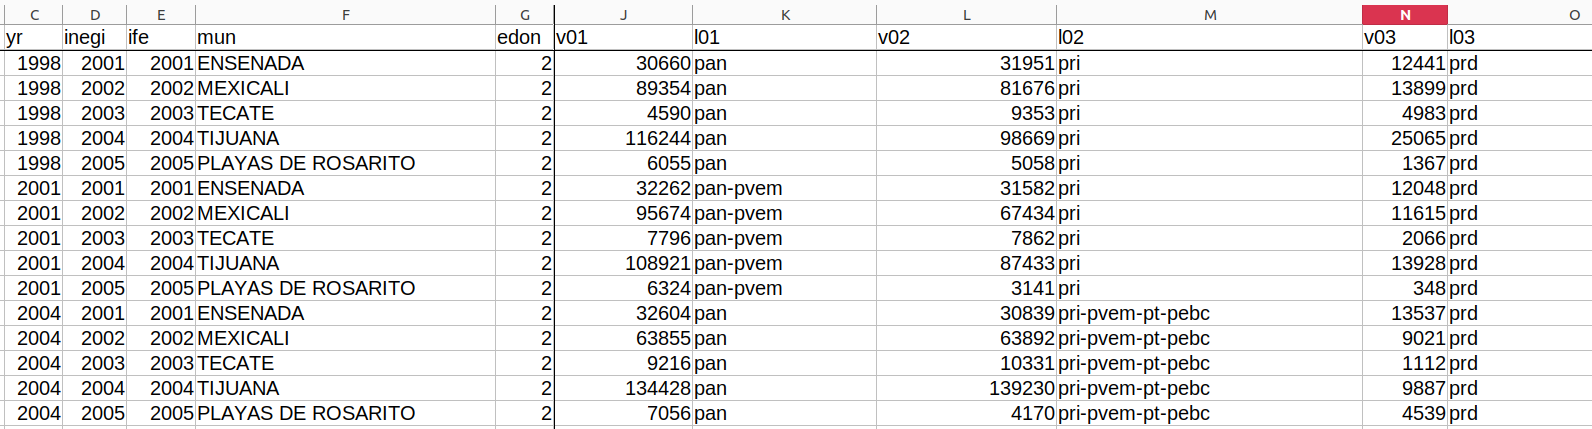
\includegraphics[width=\columnwidth]{pics/eg-spreadsheet-columns.png}
  \caption{Screenshot with a sample of the data organization}\label{F:scrn}
\end{figure}  

Figure \ref{F:scrn} offers a glimpse of the data for the state of Baja California's five municipalities in three election cycles: \verb|yr=|1998, 2001, and 2004. Two official municipal ID codes are reported: the census bureau's (field \verb|inegi|) and the electoral board's (field \verb|ife|). Those who wish to further incorporate census information or vote returns of other races into the analysis will rely on these codes for merging the data. Municipal vote returns are stored in column pairs \verb|(v01,l01)|, \verb|(v02,l02)|, etc.\ for the first candidate reported, the second candidate, and so forth. The \verb|l| column of the pair identifies the candidate's party or coalition label, while the \verb|v| column contains the total votes the candidate won. So in 1998 in Ensenada, with 31,995 votes the PRI was the plurality winner ($\texttt{l02} = \texttt{pri}$ indicates that this party's vote is stored in field $\texttt{v02}$), trailed closely by the PAN's 30,660 votes (in field $\texttt{v01}$). The votes--label column pair storage accommodates four decades of state party system heterogeneity, compounded by ephemerous electoral coalitions in a relatively small number of spreadsheet columns. The trade-off is that inspecting one party's performance across municipalities often requires additional manipulation, in order to arrange its votes into the same column across units.\footnote{A standalone R script (still a beta version) extracts a simplified matrix, reporting each party's votes in a column that is named after it, for a single state-year's municipal races. The script is located in \verb|code/extract-state-yr-mu-returns.r|.} %\emm{Should write standalone Python script too.} 

\section{Pre-election coalitions}

One obstacle to analysis are electoral coalitions. Mexican election law distinguishes two forms of pre-election coalitions that parties may choose from: joint candidacies and coalitions proper. Voters in the former case can cast their vote for any joint-candidate-nominating party (or combinations of them), which are then added up to determine the candidate's vote total. In coalitions proper, voters cast their vote for the team as a whole, which is reported with no breakdown among the coalition-member parties.

These legal subtleties have effects in public party finance mostly, but substantially complicate voting studies because scholars need to decide how to handle coalitions. To ease this decision, the repository distributes three separate municipal vote files: 

\begin{itemize}
\item \verb|data/aymu1970-on.coalAgg.csv| systematically aggregates joint-candidate coalition votes, reporting the candidate's total vote as a single quantity;
\item \verb|data/aymu1970-on.coalSplit.csv| breaks down coalesced parties' contribution to the candidate's vote total, relying for this purpose on the relative votes each party received (where the ballot structure offers this information), or on the coalition agreement between the parties (where available and when the ballot structure does not offer the latter option), or on the relative votes that coalesced parties received the last time they ran separately in the municipality (when the previous alternatives are impracticable); and
\item \verb|data/aymu1970-on.csv| has raw votes, as reported in the primary source (i.e., a vote aggregate for coalitions proper and coalition-member-party breakdowns for joint candidacies).
\end{itemize}

\noindent The files include records for the exact same set of observations and report the same total effective votes.\footnote{Or near same total effective votes: whenever the primary source does not offer the coalesced-parties vote breakdown, one artifical vote is added to the raw file, itself split among these parties to keep track of relative contributions.} Files change in how coalition votes are reported only. The typical analyst will choose between the \verb|coalAgg| and the \verb|coalSplit| files. Those interested in who won the race with what margin will prefer \verb|coalAgg|. Those wishing to study first differences in party support will opt for \verb|coalSplit|.

\begin{table}
\resizebox{\textwidth}{!}{
  \begin{tabular}{lrrrrrrrrrrrrc}
    & \mc{12}{c}{Coalition profile relative frequency (\%)} & \\ [-1.8ex]
    \\ \cline{2-12}
    \\ [-1.8ex]
     &      &              &            &            &&   \mc{3}{c}{Double-major}                    &&             &                &       &            \\ \cline{7-9}
     &      & \mc{3}{c}{Major-minor}                 &&               &    \& major-  & \& two       && \mc{2}{c}{Triple-major}      &       & (Mean co- \\\cline{3-5}\cline{10-12}
Cycle&  None&  One         & Two        & Three      &&   Only        &       minor   & maj.-min.    && Only        &  \& maj.-min.  & Total & alitions)  \\ 
     &      &              &            &            &&               &               &              &&             &                &       &            \\ [-1.8ex] \hline
     &      &              &            &            &&               &               &              &&             &                &       &            \\ [-1.8ex] 
 1979--81& 100.0&   ---&    ---&    ---&&    ---&       ---&         ---&&  ---&       ---& 100 & (0.00) \\
 1982--84& 100.0&   ---&    ---&    ---&&    ---&       ---&         ---&&  ---&       ---& 100 & (0.00) \\
 1985--87& 100.0&   ---&    ---&    ---&&    ---&       ---&         ---&&  ---&       ---& 100 & (0.00) \\
 1988--90&  93.9&   6.1&    ---&    ---&&    ---&       ---&         ---&&  ---&       ---& 100 & (0.06) \\ \hdashline
 1991--93&  98.6&   1.3&    ---&    ---&&    ---&       ---&         ---&&  ---&       ---& 100 & (0.01) \\
 1994--96&  99.8&   0.2&    ---&    ---&&    ---&       ---&         ---&&  ---&       ---& 100 & (0.04) \\
 1997--99&  96.4&   2.1&    ---&    ---&&    1.5&       ---&         ---&&  ---&       ---& 100 & (0.04) \\
 2000--02&  77.0&  16.7&    1.8&    ---&&    4.0&       0.4&         ---&&  ---&       ---& 100 & (0.29) \\ \hdashline
 2003--05&  52.8&  29.8&   11.8&    0.4&&    1.8&       3.3&         ---&&  ---&       ---& 100 & (0.65) \\
 2006--08&  20.4&  48.1&   30.2&    0.6&&    0.1&       0.7&         ---&&  ---&       ---& 100 & (1.19) \\
 2009--11&  11.2&  32.3&   14.6&   10.4&&    7.7&      23.8&         ---&&  ---&       ---& 100 & (1.54) \\
 2012--14&   8.6&  50.7&   11.6&    3.6&&    3.5&      22.0&         ---&&  ---&       ---& 100 & (1.39) \\ \hdashline
 2015--17&  24.6&  35.6&   11.0&    0.8&&    6.1&      21.7&         ---&&  0.2&       ---& 100 & (1.16) \\
 2018--20&   6.3&  17.3&   14.7&    7.1&&    6.5&      35.1&        12.9&&  ---&       ---& 100 & (1.86) \\
 2021--23&  26.8&  18.5&    0.2&    ---&&   13.0&       9.5&         0.3&& 18.2&      13.6& 100 & (1.05) \\
 2024--26&  17.4&  19.6&    1.6&    ---&&    6.1&      12.8&         0.7&& 17.1&      24.8& 100 & (1.30) \\ 
         &      &      &       &       &&       &          &            &&     &          &       &        \\ [-1.8ex] 
  \hline
\end{tabular}
}
\caption{Coalitional profile of municipal races by federal election cycle. Cells report the percentage of municipalities in the cycle, and the cycle's mean number of coalitions per race in parentheses. Quantities consider coalitions where one partner at least was a major party (PAN, PRI, PRD, or Morena), ignoring coalitions among minor parties only, which were also quite frequent.}\label{T:coal}
\end{table}

Banned until the mid-1980s at the local level, and rarely authorized up to the mid-1990s, coalitions have since become a staple of Mexican elections, as Table \ref{T:coal} shows. Each table row reports the coalitional profiles observed across municipal races in a triennium. With few exceptions owed to state electoral calendar shifts,\footnote{Subnational electoral calendars varied substantially up to 2015, but have since become increasingly aligned with the federal cycle. See \url{https://github.com/emagar/calendarioReelecion}. Change is discernible in how municipal vote shares align vertically in the right of Figure \ref{F:vpcts}, increasingly clustered over darker and distincter columns that correspond with federal elections.} triennial aggregates capture one periodic election per municipality. The coalitional profile is `None' in the absence of any coalition in the race; it is a `major-minor' arrangement when one, two, or three major parties (i.e.\ PAN, PRI, PRD, or Morena) nominated a municipal ticket jointly with one or more minor parties; it is `Double major' when two majors ran jointly; and so forth. Three distinct moments can be distinguished. (1) Between the 2000--02 and 2006--08 triennia, inclusive, at least one major party, and increasingly two major parties, would team up with minor parties to gain an edge in the municipal race. By the end of this first moment, four out of five municipal elections had one or more major-minor arrangements. (2) Between 2009--11 and 2012--14, adding frequent `double-major' races, when PAN and PRD forged anti-PRI tickets in over one-fifth of municipalities. Races without any coalition races became ever rarer. (3) Morena's foray into the party system, especially after 2018, forced frequent full regroupments of erstwhile rivals PAN, PRI, and PRD (`triple-major' coalitions) against the new Behemoth. Regroupments shrank the number of coalitions per municipality by widening their scope (the right-most column reports triennial average coalitions per municipality, parenthesized).

% And the right-most column reports triennial average coalitions per municipality, parenthesized. The mean number of coalitions only surpassed one by 2006--08, up from 0.29 six years before, and rose to a maximum 1.85 in 2018--20. It has declined since.

\begin{figure}
  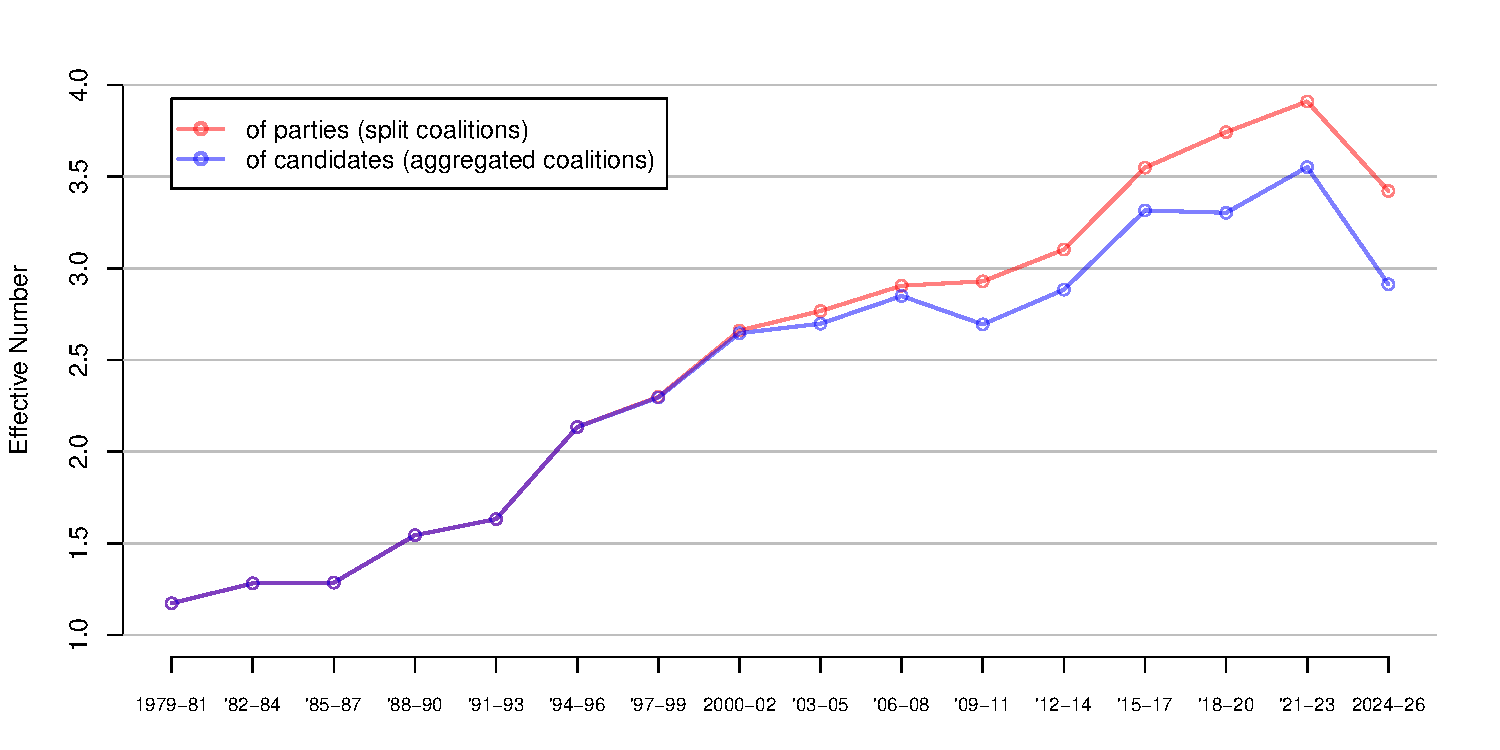
\includegraphics[width=\columnwidth]{../../plots/enp1979-2025.pdf}
  \caption{Municipal party system fragmentation by federal election cycle. Circles report the mean effective number of parties across municipal elections in the cycle.}\label{F:enp}
\end{figure}

% \begin{table}
%   \centering
%   \begin{tabular}{lcc}
%           & \mc{2}{c}{Mean effective number of}     \\ [-1.8ex] 
%     \\ \cline{2-3}
%     \\ [-1.8ex] 
%           & candidates & parties \\
%     Cycle & (aggregated coalitions) & (split coalitions) \\
%     \\ [-1.8ex] \hline 
%     \\ [-1.8ex] 
%  1979--81 &    1.17    &    1.17 \\
%  1982--84 &    1.28    &    1.28 \\
%  1985--87 &    1.29    &    1.29 \\
%  1988--90 &    1.54    &    1.54 \\ \hdashline
%  1991--93 &    1.63    &    1.63 \\
%  1994--96 &    2.13    &    2.13 \\
%  1997--99 &    2.30    &    2.30 \\
%  2000--02 &    2.65    &    2.66 \\ \hdashline
%  2003--05 &    2.70    &    2.77 \\
%  2006--08 &    2.85    &    2.91 \\
%  2009--11 &    2.69    &    2.93 \\
%  2012--14 &    2.88    &    3.10 \\ \hdashline
%  2015--17 &    3.32    &    3.55 \\
%  2018--20 &    3.30    &    3.74 \\
%  2021--22 &    3.55    &    3.91 \\
%  2024     &    2.92    &    3.47 \\
%     \\ [-1.8ex] \hline
%   \end{tabular}
%   \caption{Municipal party system fragmentation by federal election cycle}\label{T:enp}
% \end{table}

Computing the \citet{laakso.taagepera.1979} index for parties (using \verb|coalSplit| data) and for candidates (with \verb|coalAgg| data) captures the magnitude of coalition incidence neatly. A gap between the measures, portrayed longitudinally in Figure \ref{F:enp}, opened after major-party coalitions normalized in 2009. In has been widening since. The distributed file trio lends flexibility to handle coalitions in municipal elections as needed for analysis.

\section{Descriptive statistics}

This section summarizes party vote shares across municipalities nationwide. It demostrates that municipal party support in the distributed files conforms to received wisdom of Mexico's atypical democratic transition \citep[eg.][]{cornelius.1996} and subsequent political national-level development \citep[eg.][]{diaz-estevez-magaloni-Poverty-book.2016}. Patterns also emerge that are distinctive of municipal-level analysis. The summaries also shed light over potential applications of the data.

\begin{figure}
  \includegraphics[width=\columnwidth]{../../plots/vpct1979-2025.pdf}
  \caption{The electoral evolution of parties in municipal races 1979--2025. Color-coded circles report one party's vote percentage in a municipal election (slightly x-jittered for visibility). Curves are the vote percentage that each party won in the median municipality across time (the trend is smoothed for clarity).}\label{F:vpcts}
\end{figure}  

Figure \ref{F:vpcts} offers a group portrait, plotting every municipal elections since 1979 for which there is data (using the split coalition file). Each minuscule, color-coded circle quantifies a party's vote percent in one municipal election---137,813 in total, for 30,633 non-missing municipal races. The hegemonic party system of the 1960s and 1970s remained much in place at the start of the series, the PRI's red circles modally anchored at 100 percent of the vote, ruling uncontested \citep{segovia.els1979}. Back then the right-of-center PAN (in blue), as well as the new entrants in the political left (in gold), achieved more than a symbolic vote percentage in a few dozen, urban municipalities only.

Opposition parties began picking up steam after the 1982 economic crash, gradually mobilizing social discontent in the electoral arena \citep{molinar.1991a,klesner.Alignment.1993}. Plot lines, which smooth the parties' vote in the median municipality over time, neatly capture the steady erosion of the PRI's electoral support and the rise of a dual opposition. PAN and left, however, manifest a slower pace in municipal elections than national events in the second half of the 1980s would suggest. This apparent anomaly owes units with massive population disparities. Ecological analyses of voting showed that the most solid predictor of opposition voting in a unit was the share of people living in cities \citep{ames.1970,lehr.1985,magar.1994}, few in number but important in size. In a rapidly urbanizing society, this correlation became a harbinger of the challenge ahead for the PRI. It also anticipated a major obstacle for newcomers, as the PRI remained a formidable competitor in enclaves of smaller, rural, low-turnout municipalities. Up to the near end of the series, only the PRI would be capable of getting out votes in numerous units that others could only dream to approach. Until the mid-1990s, the median municipality was firmly planted in such enclaves.

\begin{figure}
  \centering
  \textbf{A -- Percent municipalities won} \\
  
\includegraphics[width=.9\columnwidth]{../../plots/pctwin1979-2025-legend.pdf} \\
  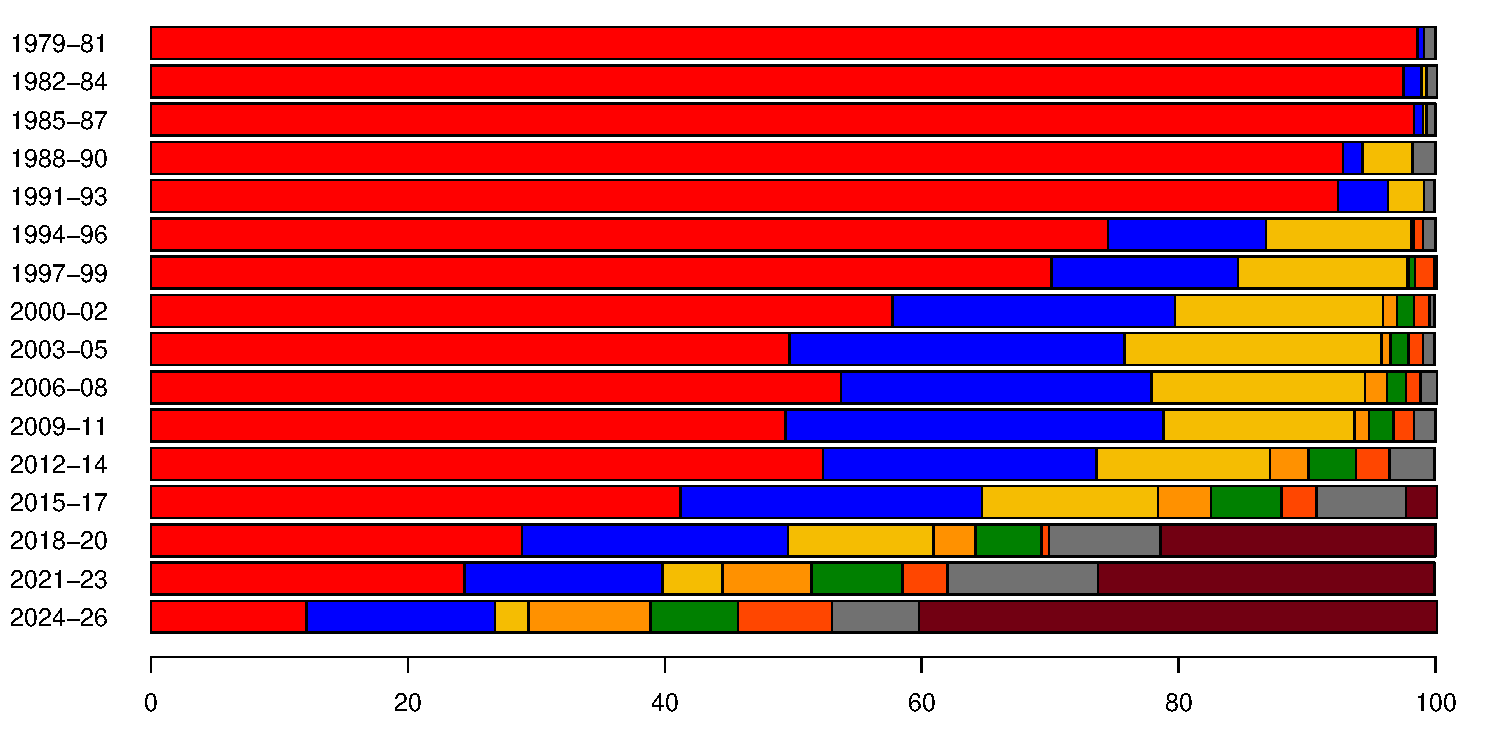
\includegraphics[width=.9\columnwidth]{../../plots/pctwin1979-2025.pdf} \\
  \textbf{B -- Size-weighted percent municipalities won} \\
  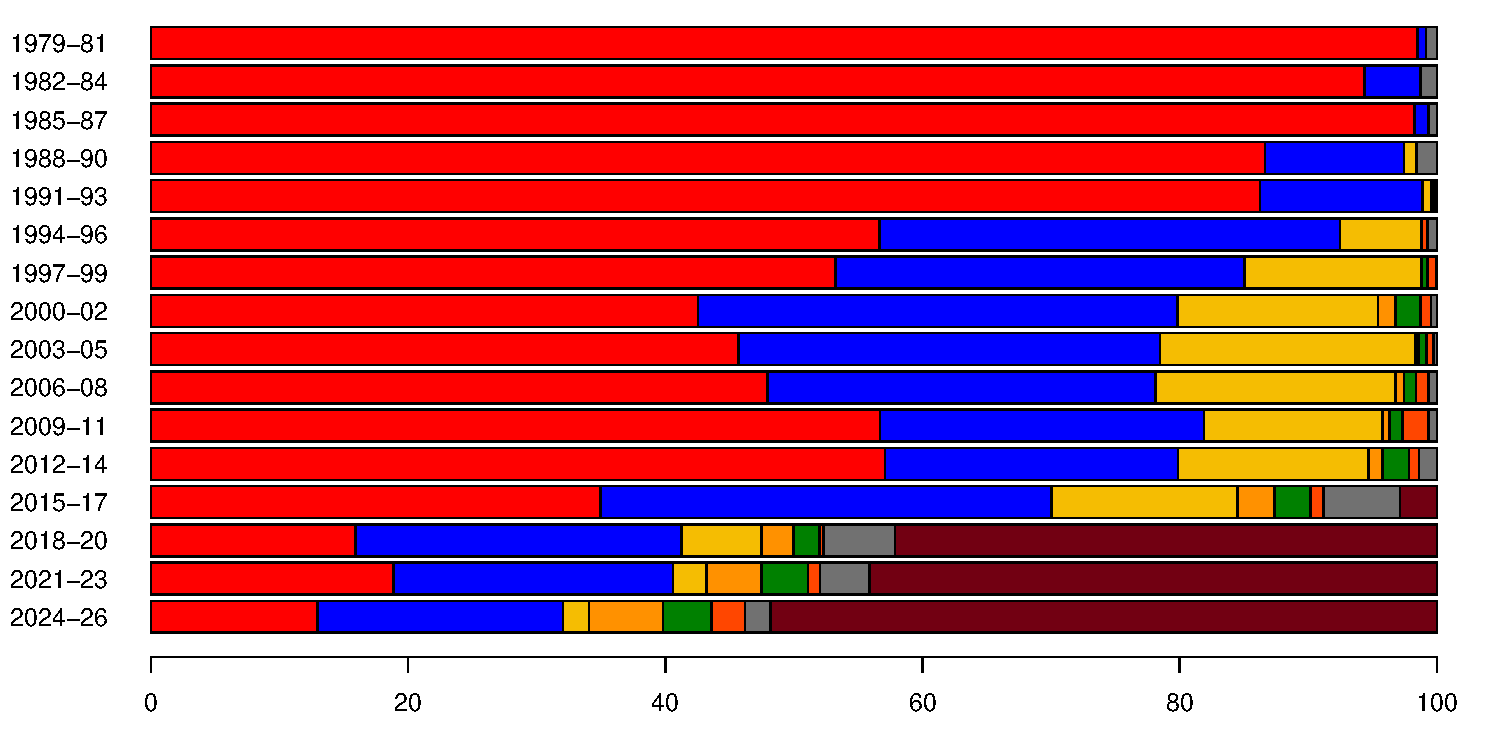
\includegraphics[width=.9\columnwidth]{../../plots/pctwin-popw1979-2025.pdf}
  \caption{Winners by federal election cycle. Relative frequencies in panel B are weighted by the municipality's population. See text on how coalition coalition victories were dealt with.}\label{F:win}
\end{figure}  

Figure \ref{F:win} approaches the lag from a slight different angle, winners in municipal races.\footnote{A separate file in the repository, \verb|data/aymu1989-on.incumbents.csv| reports the names of the winning candidates to municipal president in races since 1989.} Each horizontal bar in Panel A reports the relative number of municipalities that each party won throughout a triennial cycle. For visual simplicity, coalition winners in each election go to the major party, and when two or three majors partnered, the winner goes arbitrarily to the largest of them in the state-cycle. The PRI won nearly every municipal race in the first three triennia in the series. Its slow collapse was barely notable as late as 1993, with subsequent drops punctuated by periods of apparent stability: nine wins out of ten in 1988--1993, then three out of four in 1994--1999, then about half in 2000--2014. Then came the final collapse, when Morena took over. Panel B weights municipalities by their share of all registered voters, thus portraying the population that different parties governed in each election cycle. Up to 2008, the PAN's bars are remarkably bigger in this panel than above, indicative of its distinctive urban bias. 

The simultaneous rise of a dual opposition in Figure \ref{F:vpcts} created a coordination problem for the anti-PRI vote, a factor that played out in extending the PRI's reign despite the loss of its hegemonic status \citep{magaloni.2006,garrido-phd.2014}.\footnote{The PAN and left's parallel paths are suggestive of what \citet{cox.1997} terms a `non-Duvergerian' equilibrium: a tie between challengers that often left the PRI invulnerable in office.} Figure \ref{F:triplot} reports the share of the three-party vote for the major parties (i.e., subtracting votes won by candidates other than the PAN, PRI, and PRD). Municipalities the PRI won uncontested are bunched at top vertex, and displacements away from that vertex measure gradual decrements of the PRI vote in favor of the PAN and/or the PRD. The ternary plot echoes a pattern also seen in federal races \citep{marquez.vsData.2014}: between 1989 (the year PRD was founded) and 2014 (the year before Morena's entry), decrements are concentrated on, or very close to either triangle side. Sure, some municipalities populate the inside, but they are relatively rare. The pattern is indicative of local two-party competition. In other words, the oppositions were regionally concentrated, the PRI facing a serious challenge of one or the other, but rarely both. So, in municipal races, the PRI's persistence was not pure opposition discoordination, but genuine strength.

\begin{figure}
  \centering
  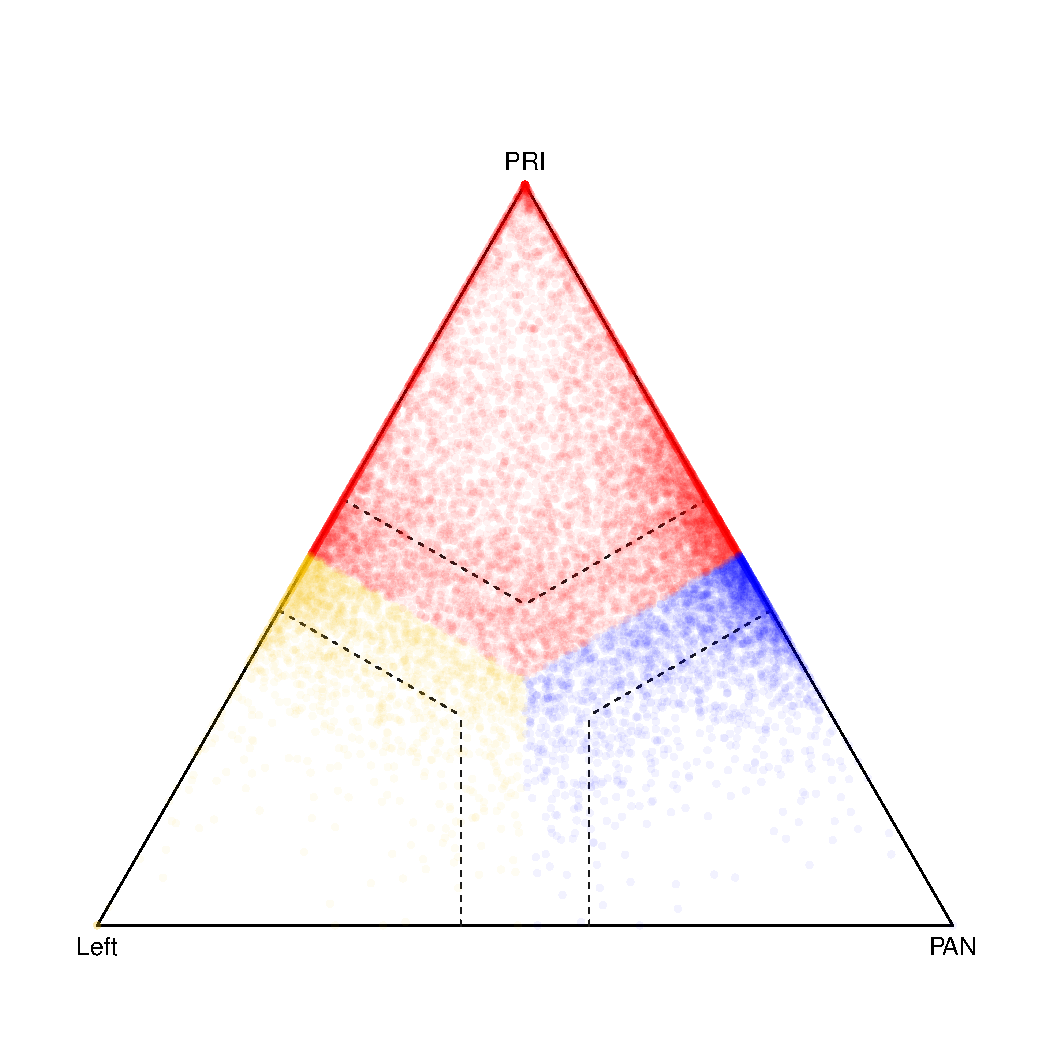
\includegraphics[width=.6\columnwidth]{../../plots/triplot1989-2014-v-mu.pdf}
  \caption{Bipartisan rivalries predominate 1989--2014. The ternary plot reports the share of the three-party vote that major parties won in municipal elections (excluding the Federal District). Points between dotted lines are marginal municipalities, where the margin between two parties was 10 percent or less.}\label{F:triplot}
\end{figure}

The final stage portrayed corresponds to the collapse of the party system that brought electoral democracy to Mexico \citep{estevez.magar.rosas.2008,moreno.decisElec.2009}, and the rise of AMLO's Morena. Andrés Manuel López Obrador, better-known by his initials, broke free from the left's proverbial factionalism \citep{bruhn.1997} by launching a new, personalized party. The gamble paid off. Left elite discoordination gave other parties unexpected victories across the board in Morena's inaugural 2015 elections. But AMLO's third bid for the presidency three years later achieved a rallying cry, becoming focal point attracting not just left voters, but independents, leaners from the PRI and even from the PAN. Morena's landslide victory in 2018, which gave it unified control of the federal and most state governments, led the former major parties to run desperate three-way coalitions in subsequent races. To little avail: while the rise of Morena appears with a lag in Figure \ref{F:vpcts} (the party mobilized the larger municipalities first, and extended its dominant mantle towards the rest afterwards), its formidable challenge managed to realign smaller municipality elites away from the PRI---the PRI's population-weighted bar in Figure \ref{F:win} finally outsized its sheer frequency in the 2024 cycle.

\section{Reelection as insurance policy}
Also discusses another dataset in the repository, incumbents. \citep{motolinia-reel-pork2021,lucardi.rosas.Incumbency.2016}

\section{The measurement of electoral history}
Also discusses another dataset in the repository, vhats.

\section{Non-fused tickets in Nayarit}
Also discusses another dataset in the repository, nayreg.





These amount to much fewer formal powers than local goverments in other systems. Mexican municipalities have no jurisdiction over public education and health, lack authority to collect other taxes, and must negotiate some fiscal resources with the state government, who may be tempted to bias redistribution of revenue sharing to municipalities \citep{timmons.broid.2013} 

Still, the institutional heterogeneity and variable socio-economic conditions make them very interesting for social science. 

But interest in Mexico's municipal government has nonetheless grown

But, with much heterogeneity, municipal governments grew in importance between 1990 and 2010. Percent of public spending they exert... making them, and the variance they manifest, attractive areas for the study of politics and policy. 






Table [[fig:1]] presents two pairs of diagrams for the 2015 (below) and 2018 (above) congressional elections. Each dot represents one municipality, colored according to the winning party, with coordinates in the ternary plot according to the relative votes of the PAN, the PRI, and the left in the federal deputy race (other smaller parties are excluded).\footnote{I must note that, for the left's electoral history (which I arbitrarily call ``Morena'' in the plots and distributed data), I systematically added up the votes of the PRD, PT, and MC up to 2015. I also added Morena's and PES's votes that year. In 2018 the left consisted of Morena, PT, and PES jointly.} 

% \begin{figure}
% \centering
% \caption{Historic expectations and municipal-level vote in two congressional elections}\label{fig:1}
% \begin{tabular}{cc}
%   \includegraphics[width=.75\columnwidth]{../assets/img/triplot2018-vhat-mu.png} &
%   \includegraphics[width=.75\columnwidth]{../assets/img/triplot2018-v-mu.png}    \\
%   \includegraphics[width=.75\columnwidth]{../assets/img/triplot2015-vhat-mu.png} &
%   \includegraphics[width=.75\columnwidth]{file:../assets/img/triplot2015-v-mu.png} \\
% \end{tabular}
% \end{figure}

The left side shows the /vote forecasts/. The idea behind this statistic is summarizing the evolution of relative votes in the municipality in five previous elections (2003--2015 in the case of 2018) and using the tendency to project a vote forecast for the current year. Plots in the right side show the actual results observed in both elections.

Three features are noteworthy in 2018. The first is the discrepancy between the left and right plots. Either the model does a poor job forecasting, or 2018 was an extraordinary election. History gave license to expect a comfortable PRI victory, both in the number of municipalities won and in margins of victory. Municipalities outside the dotted bands are won by margins of 15 points or more, and the bulk of secure municipalities are red in the forecast, with Morena in a distant second place. In fact, although a significant number of municipalities migrated towards the PAN, it was Morena who showed a clear advantage. PRI was the underachiever. In contrast, the lower left and right plots reveal fewer differences between them---2015 was a more normal election, the past offering much better grounds to forecast. 

Second, observed municipalities fled the edges and triangle vertices in 2018. Observations in vertices show a party that has no significant challenger. While those on the edges were bipartisan, whether more (inside dotted bands) or less (outside the bands) symmetric. It is also plain in forecasts that only the PAN--Morena edge was expected to be unpopulated. In practice, however, third party vote rarely collapsed to zero, there was much more dis-coordination than in the past. In fact, the intersection of dotted bands appeared denser and more homogeneous in the right than the left diagram. 

Third, the PAN /vs/ left competition was legal tender in 2018. The pattern in competitive municipalities in the last two decades, still visible in the 2015 plots, involved either PRI--PAN or PRI--left rivalries, and rarely PAN--izquierda. It was this pattern that eased electoral alliances between PAN and PRD in sub national races since 2010 that culminated in the Frente they formed in 2018 to nominate a joint presidential candidate. 

% # #+CAPTION: Una elección más característica de la partidocracia
% # #+NAME:   fig:2
% # | file:../assets/img/triplot2015-vhat-mu.png | [[file:../assets/img/triplot2015-v-mu.png]] |


% # #+CAPTION: Grano más fino: las secciones
% # #+NAME:   fig:3
% # | file:../assets/img/triplot2015-v-se.png | [[file:../assets/img/triplot2018-v-se.png]] |

Plots in Table [[fig:4]] report /secciones electorales/ and therefore offer much finer-grained than the previous portraits. They introduce the other quantity of interest in this note: parties' /core support/. The idea behind this statistic is measuring the size of the group that has historically supported the party consistently, in good but also in bad years. 

% #+CAPTION: Support core and party performance in 2018
% #+NAME:   fig:4
% | file:../assets/img/resid-pan-2018-vs-pan-core-se.png | [[file:../assets/img/resid-morena-2018-vs-morena-core-se.png]] | file:../assets/img/resid-pri-2018-vs-pri-core-se.png |

The horizontal axis in each plot measures the size of party core support groups as a proportion of the /sección/'s electorate. The PRI enjoyed a clear edge over the rest of the parties in the period, with sizable cores in /all/ secciones nationwide. The distributions of the PAN and the left, in contrast, appear concentrated towards the zero---they have relatively few secciones with some unconditional support. 

The vertical axis reports the three parties' performance in 2018 (the difference between the observed vote and the forecast). Positive values indicate that the party excelled expectations in the /sección/, negative ones that it under-performed it expectation. The PRI's electoral disaster appears all too clearly in the red plot. There were a few secciones with positive performance, but the density concentrates massively below the horizontal zero line, something that Table [[fig:1]] had hinted. What is truly remarkable is that the dismal performance is directly proportional to the size of the PRI core. President Peña and candidate Meade achieved what seemed, if not impossible, extremely improbable: they alienated the PRI's unconditional voters in 2018. The PAN and the left met expectations in secciones where they have enjoyed with groups of support. Both (especially Morena) over-achieved where they lack important cores, taking away PRI voters. 

The note elaborates how statistics were prepared (replication code can be found [[https://github.com/emagar/mxDistritos/code/elec-data-for-maps.r][here]]).

% # [[file:https://github.com/emagar/elecRetrns/raw/master/graph/nytAmloPlusAnayaPlusMeadeNegPenaWon.svg]]

% # #+CAPTION: PAN
% # #+NAME:   fig:6
% # #+ATTR_HTML: style="float:right;"
% # #+ATTR_HTML: :width 50%
% # [[file:../assets/img/resid-pan-2018-vs-pan-core-se.png]]

* First differences
One common approach to study electoral change is through first differences. Denoting $v_t$ the party's vote share in the municipality or the /sección/, in period $t$, the first difference is simply $d_t = v_t - v_{t-1}$. 

$d_t$ is an intuitive quantity, showing the sign and magnitude of change from one election to the next. But, precisely because it compares pairs of consecutive elections only, it misses more dynamic processes in the units. One example, well documented by electoral sociology, is the regression to the mean \citep{campbell.1991,segovia.els1979}. Its detection requires observing the unit through at least three consecutive periods to verify contrary signs in $d_{t+1}$ and $d_t$. The study of secular change in the Mexican party system in the last quarter of century calls for deeper historical perspective. 

(First differences appear in the fields ~d.pan~, ~d.pri~, and ~d.morena~ in the distributed data.)

* The recent linear tendency
One way of adopting it is with /vote forecasting/ from tendencies discernible in the previous five congressional races \citep{magar.gubCoatMx.2012}. I summarize the central tendency of the recent historical vote by means of linear estimation in time, fitting a straight line for each year analyzed and each party in the municipality or /sección electoral/. 

The slope of the fitted line (the tendency) serves to extrapolate the party's electoral support to the future. For instance, to get the vote share that the recent past predicts for a party in unit $u$ for 2018, I estimate the following equation 

\begin{equation}
v_{ut} = a_u + b_u \times t + \text{error}_{ut}, \; t = 2003, \ldots, 2015
\end{equation}\label{ts-eq}

that I then use to predict $\hat{v}_{u2018} = \hat{a}_u + \hat{b}_u \times 2018$. This is an out-of-sample prediction of the party's vote share, it can be compared to the party's actual vote share in 2018 to gauge whether or not the unit approximates the historical record. For the 2015 forecast the sample shifts one period to become $t = 2000, \ldots, 2012$, and so on an so forth for previous years. I distribute forecasts for 2009, 2012, 2015, and 2018, which involved fitting about 10 thousand municipal regressions and more than 250 thousand sección-level.

(Vote forecasts appear in the fields ~vhat.pan~, ~vhat.pri~, and ~vhat.morena~ of the distributed data.)

* The party's support core
The other historical statistic is the parties' core support in the unit. Its definition stems from classifying voters in three categories: (1) support groups, that in the past have consistently supported the party; (2) opposition groups, that have consistently supported another party; and (3) swing groups, that have neither consistently supported nor consistently opposed the party \citep{cox.mccubbins.1986}. The party core consists of the support groups. 

I use the procedure by Díaz Cayeros /et al/. (2016) to estimate this core. If $\bar{v}_t$ denotes the party's mean support across all units in period $t$,\footnote{The analyzed unit $u$ should be dropped from period $t$'s mean in order to not include the dependent variable in the right side of equation \ref{ts-eq}. I do not drop it due to the large number of municipal or seccional units (each contributing a fraction to the mean) and the use of vote shares (so large units are watered down): this refinement's impact should be negligible in each mean value.} for each party in each unit I fit

\begin{equation}
v_{ut} = \alpha_u + \beta_u \times \bar{v}_t + \text{error}_{ut}, \; t = 1994, \ldots, 2018.
\end{equation}\label{alpha-eq}

$\beta_u$ measures the effect that national party tides have on the party's vote in unit $u$. For instance, $\hat{\beta}_u=1$ estimates that for every percentage point that the party wins or loses nationally in year $t$, it also wins or loses one percentage point in the unit; $\hat{\beta}_u=0$, on the other hand, would indicate the unit's full isolation form national swings. It is therefore a measure of party volatility in the municipality or /sección/ (analogous to \href{https://www.investopedia.com/terms/v/volatility.asp}{"beta volatility"} in the financial literature). 

The $\alpha$ coefficient estimates the core size: expected support in unit $u$ in the hypothetical case that the party receives no vote at the national level. For instance, $\hat{\alpha}=.4$ would indicate that, in the starkest of scenarios, 40% of the electorate in the municipality is unconditional to the party---which would indeed be a core of substantial size.

A critique that can be anticipated towards this measure of the party's support core is its extreme counter-factual nature \citep{king.zeng.counterfactuals2006pa}. It deserves rigorous scrutiny, something I plan doing in the near future. 

(The parties' core support appears in the fields ~alphahat.pan~, ~alphahat.pri~, and ~alphahat.morena~ of the distributed data. Party volatility in ~betahat.pan~, ~betahat.pri~, and ~betahat.morena~.)

* Compositional variables
I close with an important feature of the model specifications, associated with the \emph{compositional} nature of electoral returns. Compositional variable are quantitative descriptions of the parts of a whole. They therefore have two characteristics: (1) they are proportions that (2) add up to unity.\footnote{Formally, the compositional are random variables subject to two constraints: 
$0 \leq v_p \leq 1 \; \forall \; p \in P \; \; and \; \; \sum_P v_p = 1.$.} 

When estimating parties separately, the challenge of equations 1 and 2 is to avoid forecasting vote shares less than zero or greater than one; and that the sum of party forecasts equals 1. To achieve this, \citet{aitchison.1986} proposes substituting vote shares by log-ratios in the analysis. Arbitrarily setting the PRI as the reference party, define party $p$'s vote relative to the PRI as 

$r_p = \frac{v_p}{v_{\text{pri}}}.$

A value $r_p=1$ would indicate a tie between the party and the PRI, while $r_p>1$ that it finished ahead of the PRI in the proportion that the value reveals. 

Thus, equation 1 is re-specified as

$\ln r_{put} = a + b \times t + \text{error}$

y equation 2 as

$\ln r_{put} = \alpha + \beta \times \bar{r}_{pt} + \text{error}.$

Applying the natural logarithm attenuates the effect of extreme values of the regressor on the dependent variable, similar as a logit regression would. Models fitting was done with ordinary least squares. 

Coefficient estimates requires transformation to collect party vote shares. Illustrating with a three-party caste, it is trivial that 

\begin{equation}
\hat{v}_p = \frac{\hat{r}_p}{1 + \hat{r}_{\text{pan}} + \hat{r}_{\text{morena}}} \; \text{and} \;
\hat{v}_{\text{pri}} = \frac{1}{1 + \hat{r}_{\text{pan}} + \hat{r}_{\text{morena}}.}
\end{equation}

%% \begin{equation}
%% \begin{split}
%% v_{\text{pri}} + v_{\text{pan}} + v_{\text{morena}} & = 1 \\
%% v_{\text{pri}} & = 1 - v_{\text{pan}} - v_{\text{morena}} \\
%% 1 & = \frac{1}{v_{\text{pri}}} - \frac{v_{\text{pan}}}{v_{\text{pri}}} - \frac{v_{\text{morena}}}{v_{\text{pri}}} \\
%% \end{split}
%% \end{equation}

These are the quantities that the distributed data report. 


% # Fácil de implementar en R:
% # a = voto partido unidad 1
% # A = voto efec unidad 1
% # N = 3 unidades
% #
% # tengo
% # v.bar = 1/3 * (a/A + b/B + c/C)
% #
% # quiero
% # v.bar.sin.aA = 1/2 * (b/B + c/C)
% #
% # hago
% # 1/3 * (a/A + b/B + c/C) =      v.bar
% #        a/A + b/B + c/C  =  3 * v.bar
% #              b/B + c/C  =  3 * v.bar - a/A
% #       1/2 * (b/B + c/C) = (3 * v.bar - a/A) * 1/2 = v.bar.sin.aA
% #
% # v.bar.sin.aA = (N * v.bar - a/A) * 1/(N-1)



\bibliographystyle{apsr}
\bibliography{/home/eric/Dropbox/mydocs/magar}


\end{document}
